\documentclass{article}

\PassOptionsToPackage{numbers,compress}{natbib}
\usepackage[dblblindworkshop]{neurips_2026}
\workshoptitle{Who Verifies the Agents? Toward Reliable Agent Development}

\usepackage[utf8]{inputenc}
\usepackage[T1]{fontenc}
\usepackage{hyperref}
\usepackage{url}
\usepackage{booktabs}
\usepackage{tabularx}
\usepackage{amsmath}
\usepackage{amssymb}
\usepackage{graphicx}
\usepackage{float}
\usepackage{xcolor}
\usepackage{microtype}
\usepackage{enumitem}

\definecolor{gerblue}{HTML}{1F5FBF}
\definecolor{gerteal}{HTML}{137B80}
\definecolor{geramber}{HTML}{B86B00}
\hypersetup{
  hypertexnames=false,
  colorlinks=true,
  linkcolor=gerblue,
  citecolor=gerblue,
  urlcolor=gerblue
}

\newcommand{\system}{\textsc{GerClaw}}
\newcommand{\claimcheck}{\ensuremath{\mathsf{ClaimCheck}}}
\newcommand{\runcommit}{\ensuremath{\mathsf{RunCommit}}}
\newcommand{\updategate}{\ensuremath{\mathsf{UpdateGate}}}
\newcommand{\placeholderfigure}[2]{%
  \fbox{\begin{minipage}[c][#1][c]{0.96\linewidth}
  \centering\small\color{gray}#2
  \end{minipage}}}

\title{\system: Three-Boundary Verification Contracts\\
for Evolvable Medical Agents}

\author{Anonymous Authors}

\begin{document}

\maketitle

\begin{abstract}
Medical-agent failures are not confined to an incorrect final answer.  A
clinical statement can lose its provenance, a stale concurrent worker can
publish a second terminal state, and an apparently improved prompt or tool can
silently regress a high-risk subgroup.  We present \system, a pre-deployment
geriatric medical-agent prototype and a reference architecture that separates
verification at three boundaries: \emph{claim}, \emph{run}, and
\emph{update}.  The current prototype partially instantiates these contracts.
Its claim path validates citation-marker ranges, records bound and unbound
medical segments, rewrites a narrow class of unsupported deterministic
diagnosis assertions, and short-circuits recognized emergencies before model
invocation; it does not establish evidence entailment or fail closed on every
clinical statement.  Its run path combines an owner lease, a monotonic
database fencing token, and an atomic terminal commit.  Its offline update
library freezes and sandboxes candidates, implements a concrete paired runner
for four routing cases, and provides signed-attestation, approval, atomic
promotion, and rollback contracts; independent sealed evaluation and a
separately authenticated approval service remain deployment requirements.
An adjacent deterministic policy suite reports 40/40 passing cases across
seven families, but does not test the run and update boundaries.  We perform
no clinical study and make no claim about diagnostic accuracy, clinical
safety, or patient benefit.  The case study argues that verification for
evolving high-risk agents should be specified as linked admission contracts
across three time scales, with implementation status exposed rather than
collapsed into a single output score.
\end{abstract}

\section{Introduction}
\label{sec:introduction}

Language-model agents interleave generated text, external retrieval, tools,
memory, and persistent actions.  ReAct-style control loops
\citep{yao2023react} and agent frameworks such as AgentScope
\citep{gao2024agentscope} make these components easier to compose, while
benchmarks expose failures in interactive environments
\citep{liu2024agentbench}.  In medicine, however, a correct-looking final
answer is only one observable at one instant.  A response can cite a source
that does not support a particular claim; a cancelled worker can finish after
its successor; or a model, prompt, retriever, or tool update can improve an
average score while degrading an elderly or high-risk slice.  Each failure can
occur even when an evaluator assigns a plausible score to the final text.

Healthcare guidance accordingly emphasizes traceability, human factors,
versioning, monitoring, and lifecycle governance
\citep{vasey2022decide,liu2020consortai,lekadir2025futureai}.  Yet these
principles do not by themselves specify which runtime objects must be
verified, when verification occurs, or what state must be committed together.
Our central position is that high-risk agent verification should cover three
objects on three time scales:
\begin{enumerate}[leftmargin=*,nosep]
    \item a \textbf{claim}, whose admissibility depends on traceable evidence
    and deterministic risk rules;
    \item a \textbf{run}, whose public outcome depends on current ownership and
    an atomic terminal state; and
    \item an \textbf{update}, whose release depends on regression checks that
    the candidate cannot observe or approve.
\end{enumerate}

We develop this position through \system, a Web-based research prototype for
older patients and geriatric clinicians.  It uses an AgentScope runtime with
retrieval, memory, governed tools, streaming output, and an operator-run
offline evolution controller.  \system\ is an instructive case because
geriatric tasks combine multimodal evidence, polypharmacy, missing or
conflicting longitudinal facts, emergency escalation, and costly failures.
The contribution is not a new clinical model.  It is a reference verification
architecture, examined against a partial implementation, in which generated
content, concurrent execution, and candidate evolution cross explicit trust
boundaries.

This paper makes three contributions:
\begin{itemize}[leftmargin=*,nosep]
    \item We define a three-boundary model---\claimcheck,
    \runcommit, and \updategate---that separates evidential validity,
    transactional finality, and update admissibility.
    \item We report implementation status boundary by boundary: citation-marker
    auditing and bounded diagnosis rewriting; lease-plus-fencing terminal
    commits; and frozen sandbox execution, a routing-only paired runner, and
    release-control contracts.  We identify independent sealed evaluation and
    approval services as unimplemented deployment obligations.
    \item We map an adjacent deterministic audit of 40 passing policy cases to
    the claims it can and cannot support.  It is not evidence for run finality,
    update admissibility, clinical effectiveness, or general safety.
\end{itemize}

The intended value is a falsifiable systems blueprint and a set of
machine-checkable obligations for the workshop community.  No human-subject
data, clinician evaluation, diagnostic-accuracy experiment, or live clinical
deployment is reported.

\section{Related Work and the Verification Gap}
\label{sec:related}

\paragraph{Agent execution and evaluation.}
ReAct couples reasoning with environment actions \citep{yao2023react},
AgentScope provides an extensible agent-development platform
\citep{gao2024agentscope}, and AgentBench evaluates agents across interactive
environments \citep{liu2024agentbench}.  ToolEmu uses an LM-emulated sandbox
to elicit long-tail risks \citep{ruan2024toolemu}; AgentDojo evaluates utility
and prompt-injection security over tool-mediated tasks
\citep{debenedetti2024agentdojo}.  These works motivate
environment-grounded testing.  Our focus is complementary: how a
deployed-style runtime makes a text segment, terminal state, and candidate
release separately admissible.

\paragraph{Evidence-grounded generation.}
Retrieval-augmented generation combines parametric generation with explicit
retrieved memory \citep{lewis2020rag}.  ALCE shows that citation correctness
and completeness are distinct evaluation dimensions \citep{gao2023alce}.
\system\ therefore does not treat the presence of a bibliography as
sufficient.  It creates validated evidence records and audits whether
detected medical segments carry an in-range marker from the current turn.
This is structural provenance, not proof that a source is medically correct
or that a claim follows from it.

\paragraph{Transactions, attestation, and assurance cases.}
Lease fencing and atomic commit are established transaction-processing
techniques rather than new consistency primitives \citep{gray1992transaction}.
Software supply-chain systems such as in-toto bind steps and artifacts to
signed attestations \citep{torresarias2019intoto}.  The ML Test Score
organizes production-readiness checks beyond predictive quality
\citep{breck2017mltestscore}, while Goal Structuring Notation makes assurance
claims, arguments, and evidence explicit \citep{spriggs2012gsn}.  \system\
draws on these traditions but applies them to three agent-specific admission
objects.  Its novelty claim is the boundary decomposition and status-aware
safety case, not fencing, signatures, regression gates, or structured
assurance individually.

\paragraph{Medical agents and clinical AI governance.}
MedAgentBench evaluates medical agents in a virtual electronic-health-record
environment \citep{jiang2025medagentbench}.  Clinical-AI reporting and
governance frameworks call for explicit intended use, human--AI interaction,
error analysis, version disclosure, traceability, and continuous stakeholder
engagement \citep{vasey2022decide,liu2020consortai,lekadir2025futureai}.
\system\ occupies an earlier, pre-clinical stage.  It translates part of that
lifecycle guidance into software invariants, while leaving clinical adequacy
to future clinician-calibrated and prospective studies.

\paragraph{Gap.}
Security benchmarks stress adversarial inputs or tool behavior, while medical
benchmarks stress task competence.  Neither perspective alone captures the
commit path of an evolving, concurrent, evidence-bearing medical agent.
Supply-chain attestation proves who produced which artifact, but not whether
a medical segment is provenance-bearing or a stale worker lost ownership.
We ask what should be checked before a runtime exposes a segment, finalizes a
run, or promotes an update, and which checks the present prototype actually
enforces.

\section{A Three-Boundary Verification Model}
\label{sec:model}

We model a turn as
\begin{equation}
R=(\tau, a, o, f, S, E, Y, z),
\end{equation}
where $\tau$ is a trace identifier, $a$ an authenticated actor, $o$ an
ephemeral lease-owner token, $f$ a monotonic fencing token, $S$ a
request-scoped clinical state, $E$ the validated evidence records, $Y$ the
private attempt outputs, and $z$ the durable terminal state.  This notation is
a reference contract, not a formal safety theorem.  Table~\ref{tab:status}
separates the target obligation from the present implementation.

\subsection{Claim admissibility}

Let $s$ be a detected medical text segment and
$\operatorname{marker}(s,E)$ indicate that the segment contains an in-range
current-turn evidence marker.  The implemented audit is
\begin{equation}
\operatorname{ClaimAudit}(s,E)=
\begin{cases}
\textsc{record-bound}, & \operatorname{marker}(s,E),\\
\textsc{record-unbound}, & \neg\operatorname{marker}(s,E).
\end{cases}
\end{equation}
For a narrow regex-defined class $D$ of deterministic diagnosis assertions,
the output sanitizer additionally applies
\begin{equation}
\claimcheck(s,E)=
\begin{cases}
\textsc{retain-text}, & s\in D\wedge\operatorname{marker}(s,E),\\
\textsc{rewrite-uncertain}, & s\in D\wedge\neg\operatorname{marker}(s,E),\\
\textsc{audit-only}, & s\notin D.
\end{cases}
\end{equation}
Thus a bound marker means structurally traceable, not semantically supported.
General medication, risk, and clinical statements are recorded but do not all
fail closed.  Before this path, deterministic red-flag patterns can produce
urgent-action guidance without a model call.

\subsection{Run finality}

Public finality is allowed only while both coordination layers agree:
\begin{equation}
\runcommit(R) =
\operatorname{ownsRedis}(o)
\wedge \operatorname{currentPG}(a,\tau,f)
\wedge \operatorname{atomic}(m,q,z),
\end{equation}
where $m$ is the assistant message and $q$ the audit event.  A worker may
stream provisional content, but it cannot publish \texttt{done} until
$(m,q,z)$ commits.  An older worker with a stale $f$ cannot write either a
successful or failed terminal state after takeover.  Attempt events remain
private; only the committed state becomes public.

\subsection{Update admissibility}

For candidate $u$ and baseline $b$, the target update contract is
\begin{align}
\updategate(u,b)={}&
\operatorname{frozen}(u)
\wedge \operatorname{sameRunner}(u,b)
\wedge \operatorname{noPublicRegression}(u,b)\nonumber\\
&\wedge \operatorname{sealedAttestation}(u)
\wedge \operatorname{humanSignature}(u)
\wedge \operatorname{atomicPromotion}(u).
\end{align}
The current concrete runner covers only \texttt{routing.strategy} with four
deterministic cases, one per required slice.  The repository defines signed
envelopes for sealed-gate facts and exact-artifact human approval, plus atomic
Git reference promotion.  It does not implement the service that runs hidden
cases or derives those facts, nor deploy the signer as a separately
authenticated authority.  Those are requirements of \updategate, not achieved
properties of the present prototype.

\begin{table}[t]
\caption{Reference obligations and implementation status.}
\label{tab:status}
\centering
\scriptsize
\begin{tabularx}{\linewidth}{@{}p{0.11\linewidth}X X X@{}}
\toprule
Object & Reference obligation & Present implementation & Not established \\
\midrule
Claim & Admit only claims satisfying an evidence policy & In-range marker
normalization/audit; diagnosis-pattern rewrite; emergency short-circuit &
Entailment and fail-closed handling of all clinical statements \\
Run & Only the current owner atomically exposes one terminal state & Redis
lease; monotonic PostgreSQL fencing; row lock; shared terminal transaction &
Tolerance of datastore or host compromise; exactly-once downstream delivery \\
Update & Same-runner regression gate plus independent evaluation and approval
& Candidate freeze/sandbox; four-case routing runner; signed-envelope and
atomic-promotion libraries & Hidden-case execution and separately deployed
evaluator/approver authorities \\
\bottomrule
\end{tabularx}
\end{table}

\subsection{Threat model and trusted computing base}

Model outputs, retrieved pages, uploaded documents, tools, and candidate
bundles are untrusted.  A runtime worker may crash, retry, or become stale; a
candidate may attempt to inspect evaluator inputs or write outside its bundle.
We trust PostgreSQL transaction and locking semantics, Redis script atomicity
for lease coordination, the controller and Docker host, protected Git
references, and uncompromised signing keys.  The run contract does not survive
database or host compromise.  Update signatures do not provide independence
if a controller can access evaluator or approval keys.  Network partitions
may reduce availability; a stale worker remains rejectable only if the
authoritative database and fencing check are reachable.  These assumptions
define the trusted computing base rather than proving safety under a fully
compromised platform.

\section{\system\ Architecture}
\label{sec:architecture}

\subsection{System context}

\begin{figure}[H]
\centering
\IfFileExists{../figures/fig1_system_overview.png}
  {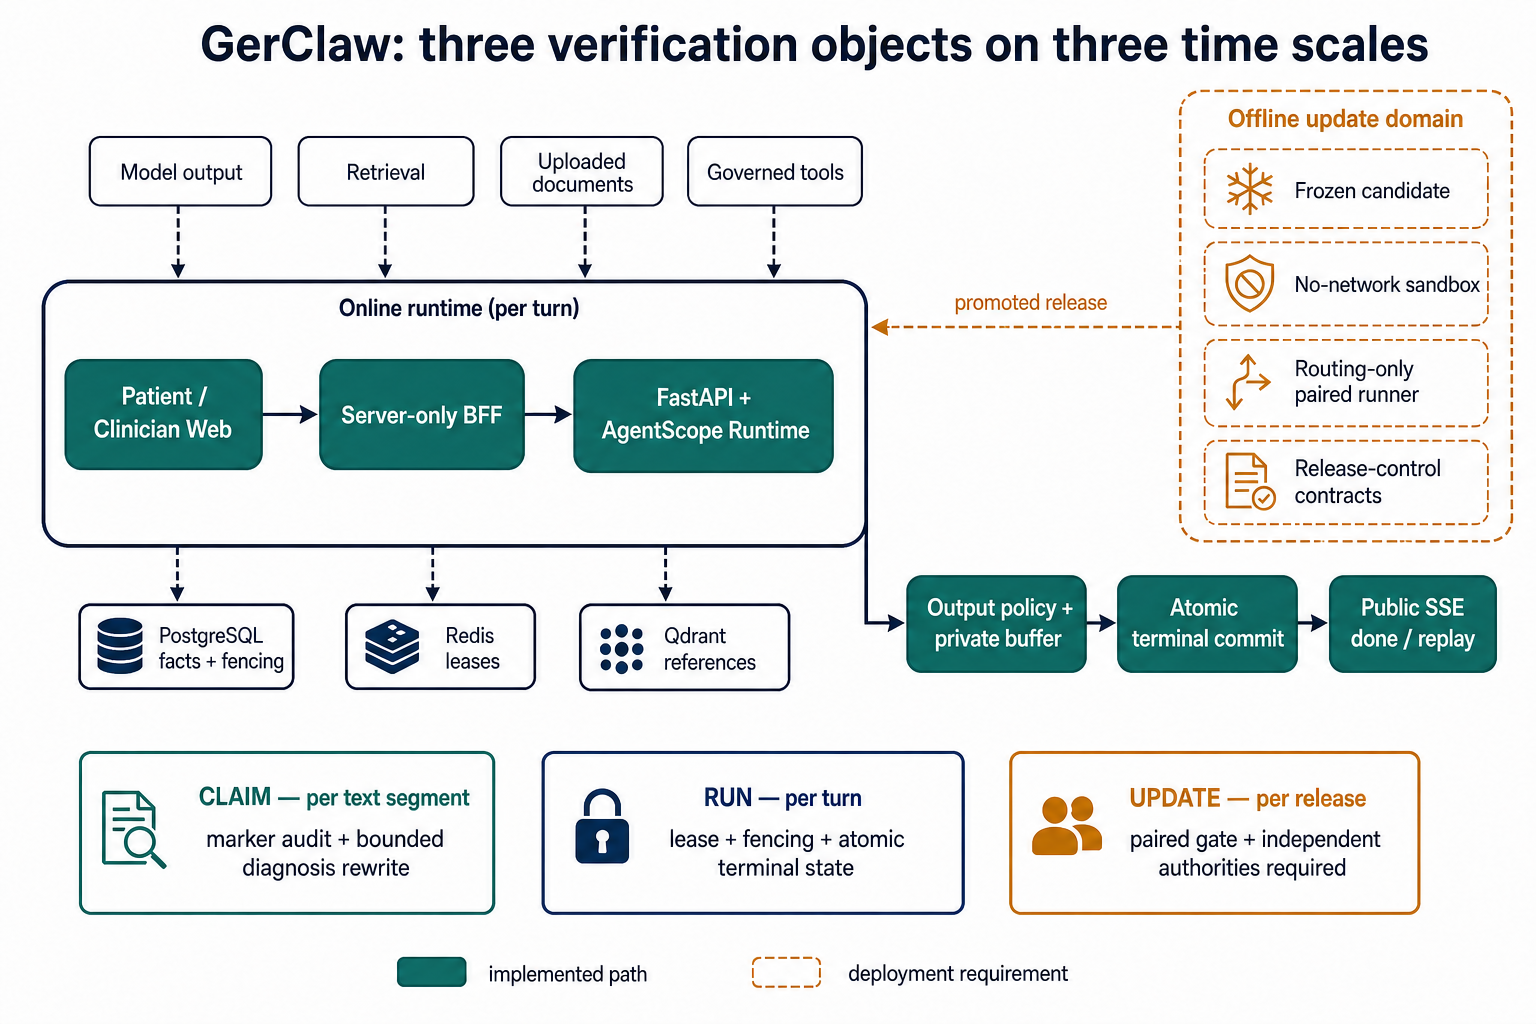
\includegraphics[width=\textwidth]{../figures/fig1_system_overview.png}}
  {\placeholderfigure{3.1cm}{Figure 1 placeholder: GerClaw system overview and
  claim, run, and update verification boundaries.}}
\caption{\system\ separates three verification objects and time scales rather
than a serial pipeline: segments are audited during generation, terminal state
is committed per run, and candidates are evaluated in an offline update
domain.  ``Verified'' denotes the named software property, never clinical
correctness.}
\label{fig:overview}
\end{figure}

\system\ separates a Web/BFF access plane, a FastAPI and AgentScope execution
plane, and durable/coordination stores (Figure~\ref{fig:overview}).  The
browser receives versioned JSON and server-sent events (SSE) but no provider,
database, or vector-store credentials.  PostgreSQL is the encrypted fact
source; Redis coordinates leases, cancellation, and short-lived guards; and
Qdrant stores retrieval and memory references that resolve back to durable
records.  Model, search, speech, parsing, embedding, and reranking providers
sit behind server-side adapters.

Each turn creates an isolated agent state.  An authenticated tenant, actor,
session, and trace scope determines which memory, documents, skills, and
tools can be composed.  The bounded ReAct loop defaults to six iterations.
Model fallback is allowed only before visible text or a tool call; the runtime
fails closed rather than splice outputs from two models after a partial
stream.

\subsection{Claim and evidence path}

\begin{figure}[H]
\centering
\IfFileExists{../figures/fig2_claim_evidence.png}
  {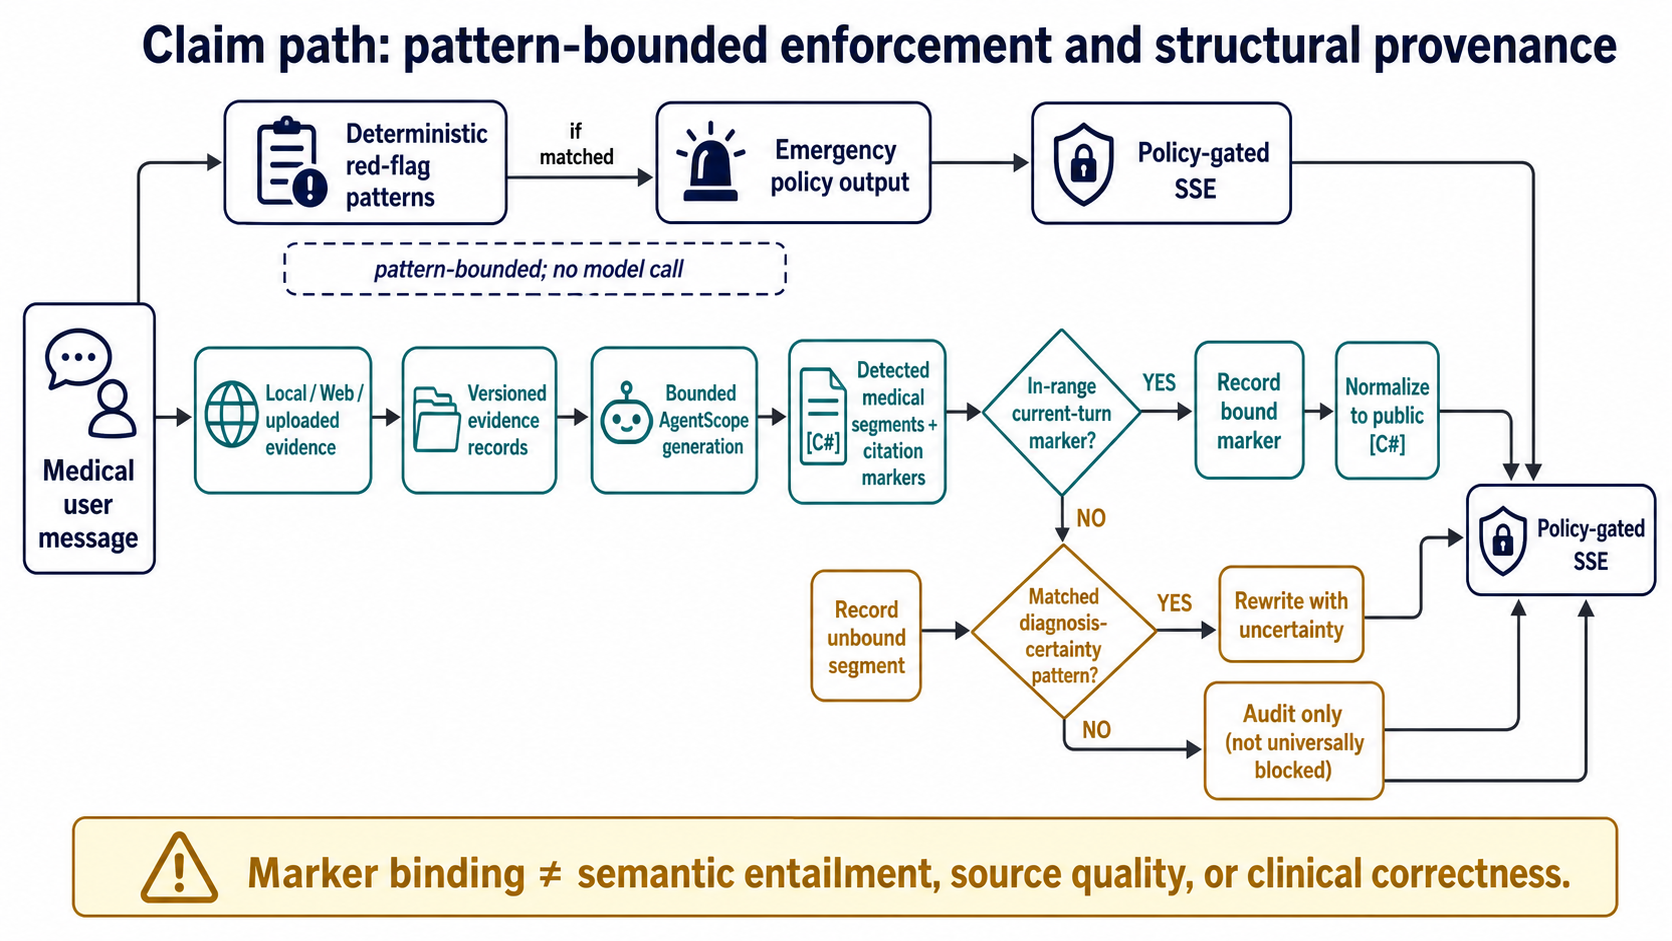
\includegraphics[width=\linewidth]{../figures/fig2_claim_evidence.png}}
  {\placeholderfigure{4.2cm}{Figure 2 placeholder: deterministic emergency
  branch and claim--evidence binding.}}
\caption{The claim path separates pattern-bounded escalation from
model-mediated generation.  It audits marker structure and rewrites only
matched unbound diagnosis-certainty patterns; other unbound segments are
recorded but not universally blocked.}
\label{fig:claims}
\end{figure}

Figure~\ref{fig:claims} shows two paths.  First, a deterministic red-flag
policy can short-circuit recognized emergency inputs, emit urgent-action
guidance, attach the uniform medical disclaimer, and close the turn without
calling a model.  This path is intentionally narrow: pattern coverage is not
equivalent to comprehensive triage.

Second, ordinary medical inputs can invoke local retrieval, governed Web
search, and tenant-scoped uploaded evidence.  Evidence responses are parsed
into versioned records before reaching the agent.  Retrieved or uploaded
content is treated as data and cannot grant tool authority.  After generation,
the output path normalizes in-range current-turn evidence markers and records
detected medical segments as bound or unbound.  For a narrow set of
deterministic diagnosis-assertion patterns, an unbound segment is rewritten
with uncertainty; other unbound clinical statements are currently audited but
not universally blocked.  The mechanism checks marker structure, not
entailment.  Patient-facing actionable conclusions receive one concise review
notice; clinician-facing output is not mechanically suppressed.

\subsection{Transactional run lifecycle}

\begin{figure}[H]
\centering
\IfFileExists{../figures/fig3_transactional_run.png}
  {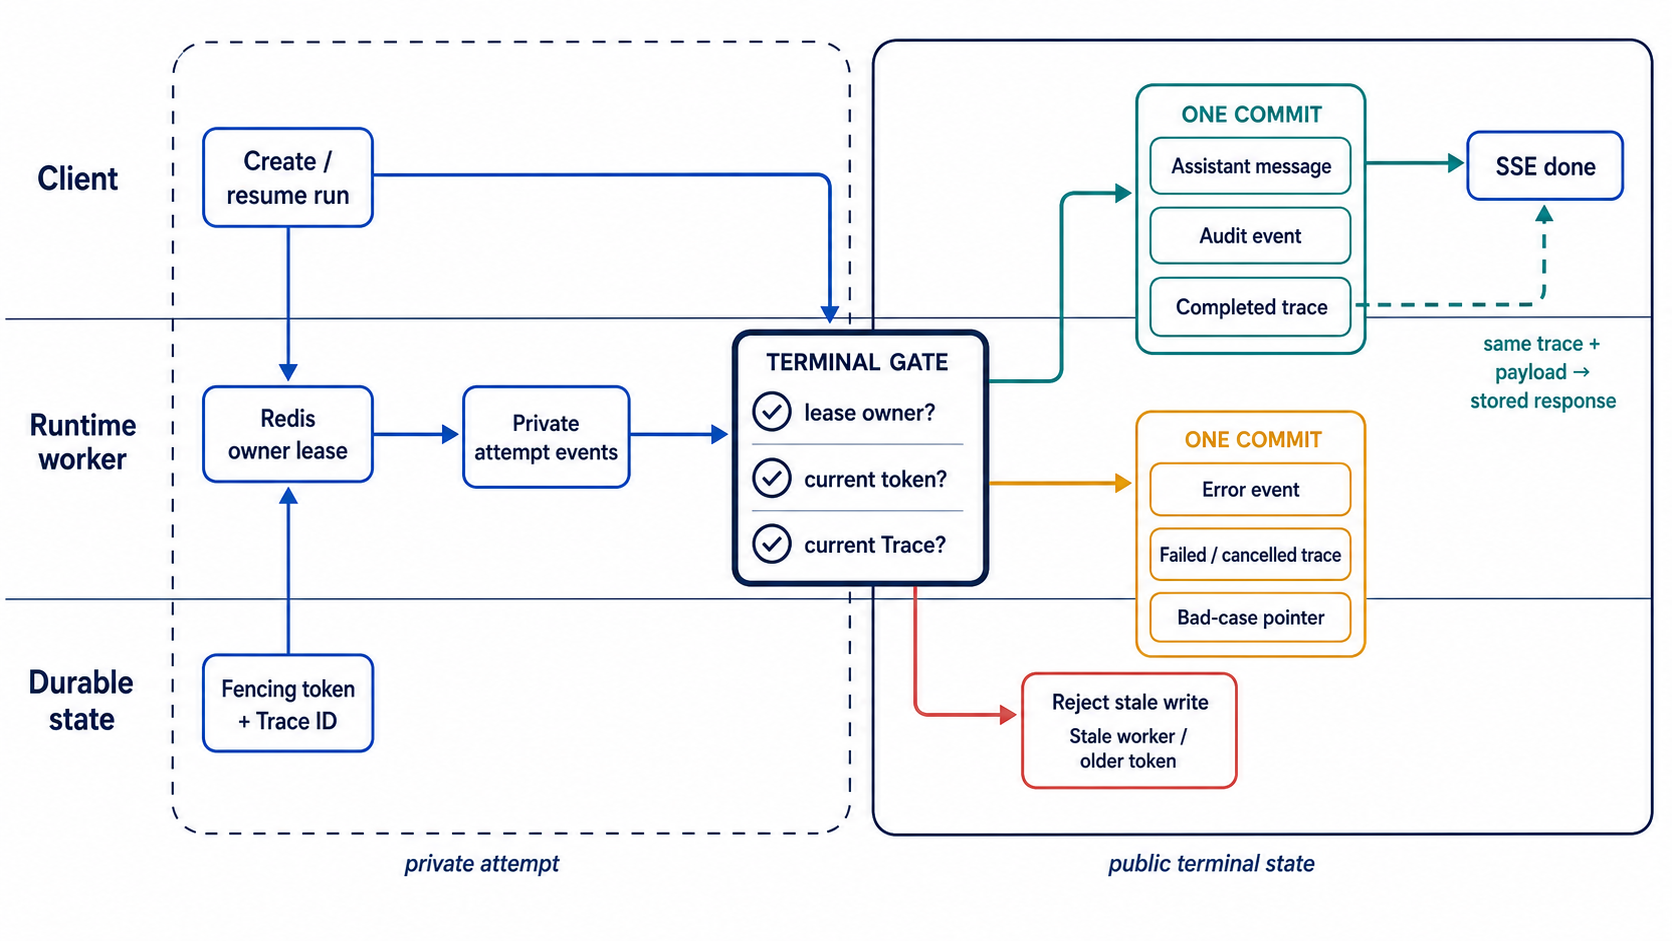
\includegraphics[width=\linewidth]{../figures/fig3_transactional_run.png}}
  {\placeholderfigure{4.0cm}{Figure 3 placeholder: lease, fencing, private
  attempts, and atomic terminal commit.}}
\caption{Run verification.  A Redis lease serializes the common case; a
monotonic PostgreSQL fencing token rejects a stale owner.  Success or failure
becomes public through one terminal transaction, and \texttt{done} follows
the commit.}
\label{fig:run}
\end{figure}

A random owner token leases a session while PostgreSQL assigns a monotonic
fencing token to each attempt.  The new owner writes its token and trace ID
before loading bounded history.  Before any terminal write, it renews and
compares the Redis owner and locks the corresponding PostgreSQL session row to
verify the token and trace.

On success, the assistant message, audit event, and completed trace share one
transaction.  On failure or cancellation, the stable public error, failed or
cancelled trace, and de-identified bad-case pointer share a corresponding
transaction.  Rollback prevents a partial terminal state.  Only after commit
does the runtime emit \texttt{done}; a completed retry with the same trace and
payload returns the stored encrypted response without a second model call.
This design does not make Redis a fact source: the database record remains
authoritative when leases expire or processes disappear.

\subsection{Governed offline evolution}

\begin{figure}[H]
\centering
\IfFileExists{../figures/fig4_offline_evolution.png}
  {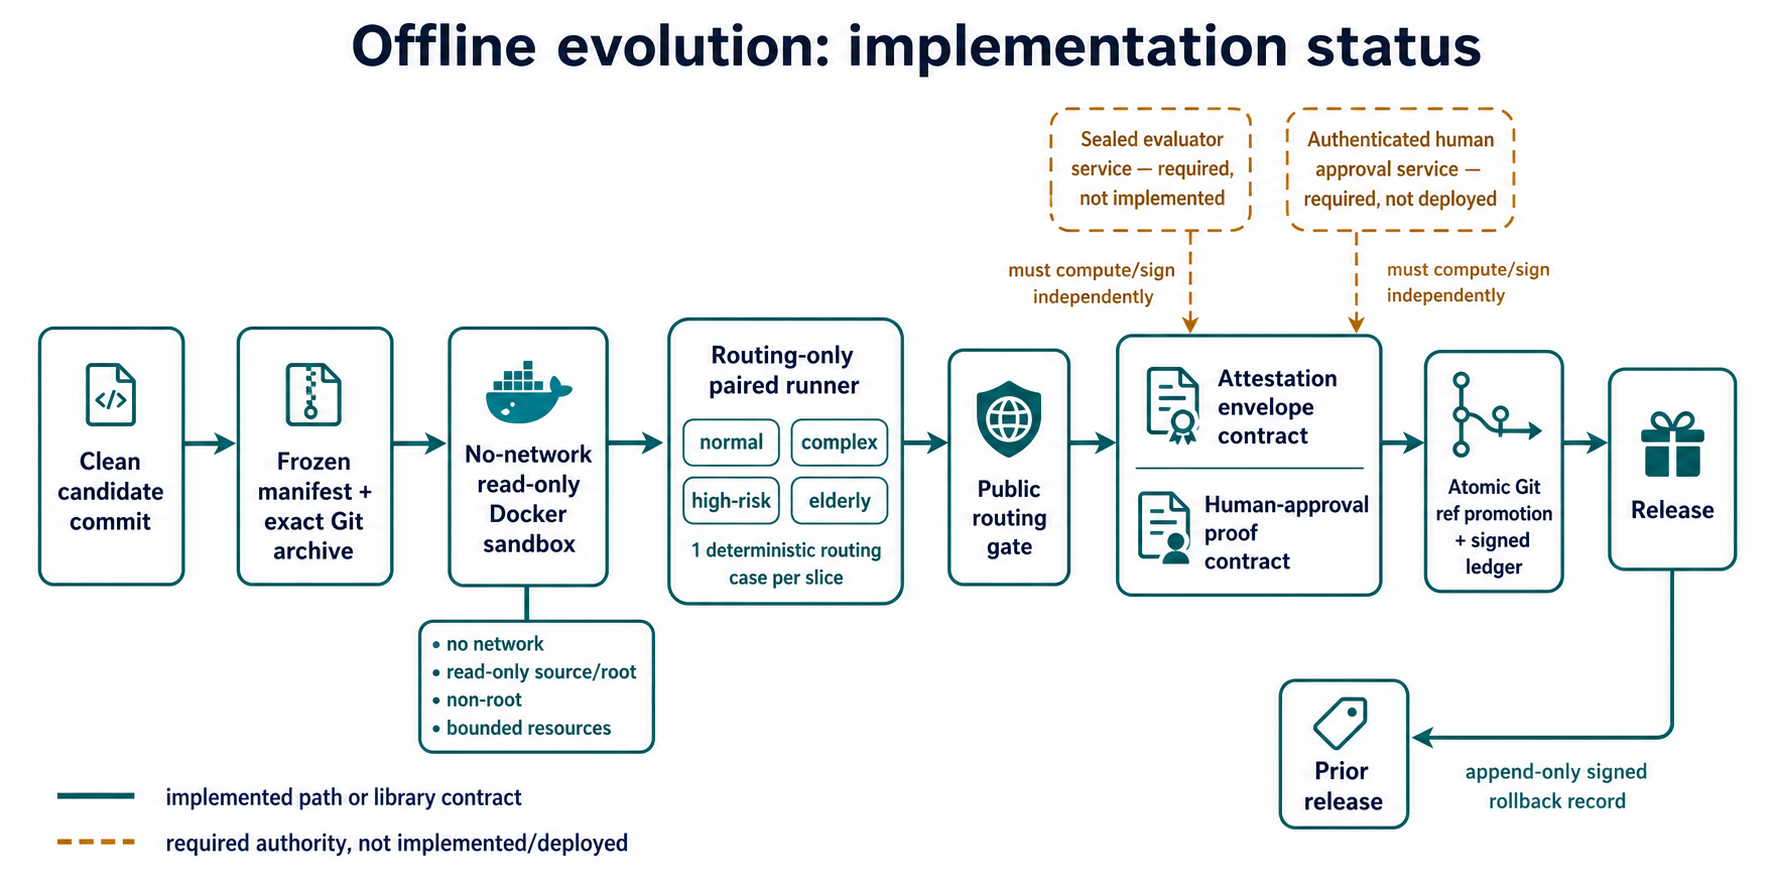
\includegraphics[width=\textwidth]{../figures/fig4_offline_evolution.png}}
  {\placeholderfigure{3.6cm}{Figure 4 placeholder: frozen candidate,
  restricted sandbox, paired and sealed evaluation, human approval, atomic
  promotion, and signed rollback.}}
\caption{Update contracts and implementation status.  Solid components are
implemented library or routing-runner paths; dashed authorities are required
for a complete deployment but are not implemented or deployed in this work.}
\label{fig:evolution}
\end{figure}

The evolution controller is an operator-run application outside the
production API image.  It accepts a clean candidate commit, freezes the
committed diff and modes, and binds every changed path to an allowed
object-kind policy.  Execution uses an exact Git archive in a
content-addressed, preinstalled Docker image with no network, a read-only root
and source, non-root identity, isolated temporary storage, bounded resources,
and verified cleanup.  The live worktree, source repository, Docker socket,
credentials, release references, and hidden tests are not mounted.

The only concrete paired runner currently accepts
\texttt{routing.strategy}.  Baseline and candidate use the same
evaluation-profile digest on four deterministic cases---one each for normal,
complex, high-risk, and elderly slices---and verify the intended router module
was activated.  This demonstrates a narrow execution path, not general agent
quality or subgroup coverage.

The control library defines two additional artifact contracts.  An
attestation envelope binds declared sealed-gate facts to an evaluator key, and
an approval envelope binds an exact candidate, reports, ticket, and trusted
time to an Ed25519 key.  The repository does not contain the independent
hidden-case runner that computes those sealed facts, and the approval signer
is a package class rather than a deployed authenticated service.  A complete
\updategate\ deployment must supply and isolate both authorities.  The
promotion library re-verifies artifacts and moves release and ledger
references in one Git reference transaction; rollback appends a signed
history entry instead of erasing the prior release.

\section{Executable Engineering Evidence and Coverage Gaps}
\label{sec:evidence}

This paper adds no research experiment.  To distinguish implemented contracts
from architectural aspiration, we executed the repository's existing
deterministic evaluation entry point:
\begin{center}
\small\ttfamily
python -m gerclaw\_api.modules.evals.cli
\end{center}
The run reported 40 of 40 passing cases.  Its JSON includes
\texttt{external\_model\_or\_rag=false}; this field is suite metadata
consistent with the deterministic call graph, not evidence from
network-egress interception.  The run used no patient data, model sampling,
retrieval, training, or parameter selection.  The internal machine-readable
audit records the command, date, counts, and interpretation, but the anonymous
submission does not include source, environment capture, or raw-output hash.

\begin{table}[t]
\caption{Composition of the existing deterministic regression suite.  Counts
are cases, not independent clinical examples.}
\label{tab:regressions}
\centering
\small
\begin{tabularx}{\linewidth}{@{}Xrr@{}}
\toprule
Policy family & Cases & Passed \\
\midrule
Emergency short-circuit and negation & 6 & 6 \\
Output-safety rewriting & 3 & 3 \\
Privacy redaction by egress purpose & 6 & 6 \\
Medication-rule contracts & 6 & 6 \\
Memory extraction and subject binding & 4 & 4 \\
Runtime security-profile admission & 12 & 12 \\
Skill-draft review coverage & 3 & 3 \\
\midrule
\textbf{Total} & \textbf{40} & \textbf{40} \\
\bottomrule
\end{tabularx}
\end{table}

The suite makes a limited but useful claim: selected adjacent policy contracts
are executable and their named positive and negative cases currently behave
as specified.  Five positive emergency cases exercise six red-flag codes,
while a negated chest-pain case does not short-circuit; malformed
direct-diagnosis outputs are rewritten; egress-purpose policies redact
labeled identifiers; known medication combinations produce versioned
findings; and runtime assets with missing budgets or version mismatches are
denied.

The suite does \emph{not} estimate sensitivity, specificity, diagnostic
accuracy, calibration, utility, fairness, latency, or clinician agreement.  It
also does not exercise stale-owner takeover, transaction rollback, unique
terminal publication, hidden-case execution, independent approval, or atomic
release promotion.  Its cases are curated software regressions and are neither
sampled from a population nor statistically independent.  A 40/40 pass cannot
be used to compare \system\ with another agent or to infer performance on
unseen language.  The evolution library has additional implementation tests,
but this paper does not aggregate them as a benchmark because no
clinician-calibrated update set or prospective protocol has been frozen.

\paragraph{Why include non-experimental evidence?}
Architecture papers can accidentally describe mechanisms that are absent from
the artifact.  The regression map makes narrow policy assertions falsifiable:
the code either admits or rejects a version-mismatched runtime asset and
rewrites the specified unsupported diagnosis-output case.  It is adjacent
engineering evidence, not an end-to-end safety case or an effectiveness
result.  External replication remains limited until an anonymous artifact can
be released.

\section{Limitations, Ethics, and Research Agenda}
\label{sec:limitations}

\paragraph{No clinical validation.}
\system\ is a research prototype, not a clinically validated system or a
medical device.  We used no patient data and enrolled no clinicians or
patients.  The work cannot support claims about diagnosis, treatment quality,
workflow benefit, trust, safety in use, or health outcomes.  A future
early-stage clinical investigation would require institutional review,
prospective protocol registration, human-factors analysis, error reporting,
and adherence to relevant guidance such as DECIDE-AI
\citep{vasey2022decide}; later trials would require an appropriate
CONSORT-AI-style design \citep{liu2020consortai}.

\paragraph{Evidence is not truth.}
Structural citation validation can show that a claim points to a current,
authorized evidence record; it does not prove source quality, retrieval
completeness, entailment, guideline currency, or patient applicability.
Moreover, the present sanitizer rewrites only matched deterministic diagnosis
phrases; other unbound clinical segments are audited but are not universally
blocked.
Image and document interpretation remain model-dependent.  The deterministic
red-flag policy covers named patterns and can miss paraphrases, languages, and
unanticipated presentations; an overly broad policy can also over-escalate.

\paragraph{Transactional assumptions.}
Lease and fencing checks depend on correct datastore isolation, durable
transactions, clock and timeout configuration, and operational monitoring.
Atomic database finality does not guarantee that every downstream consumer
observes events exactly once.  The external audit mirror for evolution can
enter a repair-required state even when the signed Git ledger commits.

\paragraph{Incomplete integration and deployment controls.}
The unified Harness currently composes memory, skills, and validated uploaded
documents in standard chat turns, but CGA, voice context, and governed
prescription workflows are not all connected through the same path.  The
release signer, human signer, sealed evaluator, protected Git references, and
audit mirror must be deployed as separate identities and trust roots.  Only a
routing-specific four-case paired runner is concrete today; the sealed
evaluator and independently authenticated approval service are not implemented
or deployed.  Repository contracts cannot substitute for an HSM, branch
protection, host permissions, or institutional approval.  The broader project
remains under active development and has not completed its final release
regression.

\paragraph{Fairness, privacy, and misuse.}
The geriatric focus creates an obligation to evaluate age-associated sensory,
cognitive, literacy, language, disability, polypharmacy, and multimorbidity
subgroups rather than treat ``elderly'' as one homogeneous slice.
Minimizing traces and separating private attempts can reduce unnecessary
exposure, but retained medical text, images, and documents remain sensitive.
Conversely, the same verification architecture could make an unvalidated
medical agent appear more trustworthy than its clinical evidence warrants.
Interfaces and publications must therefore distinguish software invariants
from clinical assurance and preserve clinician oversight.

\paragraph{Next evaluation.}
A credible next study should freeze synthetic, clinician-authored geriatric
case families; reserve a sealed family-level test set; mutate prompts, models,
retrievers, rules, and tools; and compare update gates on critical-safety
regression, task utility, over-refusal, evidence entailment, and subgroup
performance.  At least two clinicians should independently define high-risk
rubrics and adjudicate blinded disagreements.  Such a study is future work,
not evidence in this paper.

\section{Conclusion}
\label{sec:conclusion}

\system\ illustrates a broader design principle for evolvable high-risk agents:
verification is not one score applied after generation.  A claim should cross
an evidence boundary, a concurrent run should cross a transactional finality
boundary, and a candidate update should cross an evaluator and human-authority
boundary.  The partial implementation makes some obligations concrete:
marker auditing and bounded diagnosis rewriting, emergency short-circuiting,
lease-plus-fencing atomic commits, frozen sandbox execution, a routing-only
paired runner, and signed release-control contracts.  Independent sealed
evaluation, deployed approval authority, broad claim enforcement, and
clinical validation remain open.  Existing deterministic regressions support
selected adjacent policies only.  Treating verification as linked,
status-labeled admission contracts clarifies both what the current system can
defend and what future systems and clinical evaluation must still establish.


\bibliographystyle{plainnat}
\bibliography{references}

\input{checklist_answers}

\end{document}
